% This is samplepaper.tex, a sample chapter demonstrating the
% LLNCS macro package for Springer Computer Science proceedings;
% Version 2.20 of 2017/10/04
%
\documentclass[runningheads]{llncs}
%
\usepackage{graphicx}

% Used for displaying a sample figure. If possible, figure files should
% be included in EPS format.
%
% If you use the hyperref package, please uncomment the following line
% to display URLs in blue roman font according to Springer's eBook style:
% \renewcommand\UrlFont{\color{blue}\rmfamily}

\begin{document}
%
    \title{A simple and Efficient Native Language Identifier\thanks{Supported by organization x.}}
%
%\titlerunning{Abbreviated paper title}
% If the paper title is too long for the running head, you can set
% an abbreviated paper title here
%
    \author{First Author\inst{1}\orcidID{0000-1111-2222-3333} \and
        Second Author\inst{2,3}\orcidID{1111-2222-3333-4444} \and
        Third Author\inst{3}\orcidID{2222--3333-4444-5555}}
%
    \authorrunning{F. Author et al.}
% First names are abbreviated in the running head.
% If there are more than two authors, 'et al.' is used.
%
    \institute{Princeton University, Princeton NJ 08544, USA \and
        Springer Heidelberg, Tiergartenstr. 17, 69121 Heidelberg, Germany
        \email{lncs@springer.com}\\
        \url{http://www.springer.com/gp/computer-science/lncs} \and
        ABC Institute, Rupert-Karls-University Heidelberg, Heidelberg, Germany\\
        \email{\{abc,lncs\}@uni-heidelberg.de}}
%
    \maketitle              % typeset the header of the contribution
%
    \begin{abstract}
        There are around 45 million native people in Latin America; 900 thousand of them live in Brazil. Despite that, there is a lake of resources for their language. Moreover, the currents translation platform like google and bing translator does not provide an automatic identification for them. Therefore, this paper gives a step toward the development of a simple and efficient method to classify the native Brazilian language automatically.
        \keywords{Languages Identification \and Natural Language Processing \and  Features Extraction \and Information Retrieval}
    \end{abstract}

%
%
%

    \section{Introduction}\label{sec:introduction}
    According to the International Labour Organisation (ILO) 169 agreement over native people; it is possible to identify a group of indigenous using some aspects.
    The considered features are the territory, identity recognition, common origin, culture, and language \cite{povos_indigenas}.
    Furthermore, according to \cite{povos_indigenas}, there are 45 million native people only in Latin American.
    It shows the significance of the study of their native languages, and the use of computational resources to make it accessible.

    Although according to \cite{povos_indigenas} there are 900 thousand native people only in Brazil, the lack of resources is one of the biggest concerns in the development of a natural language processing method to native languages.
    Once the languages like the ones from Tupi have an oral tradition;
    there are only a few texts available for computational analyses.

    Moreover, some of the languages native of Latin American, have a poly-synthetic nature, it means that one single word can represent a whole clause, and the Tupi is one of them \cite{lemos1956tupi}.
    This same issue was faced on~\cite{kann2018fortification} study.
    The discovered technique to handle this difficulty was to divide the words in the smallest morphological component providing a more extended and varied vocabulary.

    Besides, computers have taken a prominent part of our lives, mainly in the day to day tasks \cite{matthews2016introduction}.
    Moreover, most of human communication uses natural language~\cite{matthews2016introduction}.
    Thus,  the development of a process to make the human language able to be understood by the computers would be of great importance~\cite{matthews2016introduction}.

    One of the resources provided by google translator is classifying a given text by the language and therefore is an excellent example of the purpose of this paper.
    It achieved using today's wide used method known as the natural language process.
    It comes from the result of the use of artificial intelligence and linguistic\cite{nadkarni2011natural}.
    Besides, it seeks to fill this gap between computer and human communication. Also, it has suffered a great explosion of works focusing on several languages groups\cite{peters2002evaluation}.


    Therefore, considering the importance of the native languages and its identification for a computational system.
    We use the tools of the natural language processing and information retrieval to identify and classify 26 Brazilian native languages and the Portuguese. Furthermore, we developed a method of easy classification that considers the lake of a priori information in many languages around the world.

    \section{Background work}\label{sec:background-work}


    The multi-language classification task has been under exploration for many years since 1967~\cite{cabral_2015}. Since then, the number of techniques has been growing in various ways to supply different demands on how a given language or set of language might be distinguished~\cite{jauhiainen2019automatic}. There are two foremost classification processes~\cite{gomez2017discriminating}. One process classifies both language and dialect in a single step. The other one first distinguishes the language and, a different subroutine recognizes the dialect in which the document belongs~\cite{gomez2017discriminating}. We can also cite the methods using linear Machine Learning (ML) algorithms such as Logistic Regression, Support Vector Machine (SVM) and ensemble classifiers, the most popular in this case~\cite{gomez2017discriminating}. In both algorithms, the features are characters n-grams and the bi-grams of words \cite{gomez2017discriminating}.

    The language classifiers can use different methods to achieve their purpose. Some of them make use of the term frequency or n-gram term frequency to identify a language or dialect ~\cite{jauhiainen2019automatic}. One example is the TextCat \cite{cavnar1994n} where each language has a specific profile based on the n-grams term frequency of pre-defined word categories. That work achieved 99.8\%
    accuracy as results classifying newsgroup articles from different language sources and in computer-oriented articles it performed, making 80\% correct prediction. The results consolidate the work as state of the art in the text classification field.

    There are some other approaches focused on the classification of a specific dialect or even similar languages instead of a language itself~\cite{jauhiainen2019automatic}~\cite{gomez2017discriminating}. It has shown to be a hard problem to deal with, but some other methods have also revealed to be helpful~\cite{jauhiainen2019automatic},~\cite{gomez2017discriminating}.

    The work~\cite{gomez2017discriminating} chose to use the SVM and Multinomial Naive Bayes classifier to predict 14 different languages correctly. They included languages of the same group as the Brazilian Portuguese and European Portuguese. They also used the language of different groups such as European French and Argentinian Spanish. They chose to make a two-step classification identifying first the group which the language might belong and secondly the language itself. Their algorithm uses the frequency of several n-grams affix configurations extracted from journalistic documents. They reached their best result having 91.6\% accuracy.

    One example using Artificial Neural Network (ANN) is the work of~\cite{kp2019deep} that uses a Long Short Term Memory (LSTM) to distinguish dialect by the character's frequency. An LSTM is an ANN able to memorize sequences of data used in some cases to the classification task~\cite{ghosh2016contextual}. That way, specifics character's chains feed the LSTM and further classify the dialect. The results presented an accuracy of 0.246 using lexical features. When they use the framework of the features' vector, the result improves substantially to 0.577.

    There are many other methods related to language identification of a specific document~\cite{jauhiainen2019automatic}. However, we wished to focus on the ones related to the frequency of the terms. Then, given an introduction to the used method in this paper.


    \section{Research Questions}

    To face the problems raised in previous section, we are interested in evaluate if it is possible to develop a classifier without prior knowledge of an specific language, that can be trained with a small dataset (since only a few documents are in digital form in Latin America native language) and using shallow text mining features (as there are no natural language processing methods available for some native languages). Therefore, this work will address the following research question.

    \begin{itemize}


        \item \textbf{To what extent can text mining methods automatically categorise native languages with a small dataset and no prior knowledge?}

%As we discussed before (see section~\ref{sec:introduction}), some language have a few or none syntactic and morphological information about them available. Thus, it is relevant to classifier them without prior knowledge.

        % \item \textbf{How to develop an algorithm able to be efficient with minimal digital text corpus availability?}

%Since only a few documents are in digital form in Latin America native language, the training algorithm cannot require big text corpora.
% \item \textbf{How simple can be the method using only term frequency?}

%  \textit{Considering the state of the art in the text classification  (see section:~\ref{sec:background-work}), we would like to explore the limits of this approach in terms of combination between simplicity and efficient.}
    \end{itemize}


    \section{Materials and Methods}\label{sec:materials-methods}
    \subsection{Materials}\label{materials}
    We obtained 27 versions of the Holy Bible in 26 native languages and one in the Brazilian Portuguese  (in the New Translation in Today's Language) available at \cite{angelo}.  The archives originally were in the \textit{.sqlite} format and were then converted to \textit{.csv}.

    Another significant aspect is that the raw document held some challenges like HTML tags inside of the scriptures; moreover, there were various cross-references in some documents. Fortunately, we got rid of all those issues~\footnote{
        We used the pandas python library tools to clean up the text (see~\cite{pandas-dev_2020}) for more information. } and obtain a clean proper text for classification. As long as no stemming algorithm is known for the 26 native languages, we used an automatic stemming procedure in subsection~\ref{subsec:stemming-procedure}.In our case, we consider only each word as a specific token for our method implementation. Furthermore, as long as just a few documents hold the whole bible scripture (Guarani Mybá, Brazilian Portuguese and Guajajara), we decided to use only the New Testament as documents for the classification to guarantee a fair outcome result.
    \begin{table}[ht!]
        \caption{This table describes the \textit{.csv}
            file that holds one of the 27 versions of the bible. The version showed is the Portuguese in the New Translation in Today's Language.}
        \begin{center}
            \begin{tabular}{|c|c|c|c|}
                \hline
                \textbf{Book} & \textbf{Chapter}& \textbf{Verse}& \textbf{Scripture} \\
                \hline
                40 & 1 & 1 & `` Esta é a lista dos antepassados... " \\
                \hline
                40 & 1 & 2 & ``Abraão foi pai de Isaque, Isaque foi... " \\
                \hline
                40 & 1 & 3 &   ``Judá foi pai de Peres e de Zera, e..."  \\
                \hline
                \vdots & \vdots & \vdots & \vdots\\
                \hline
                66 & 22 & 21 & ``E que a graça do Senhor..." \\
                \hline
            \end{tabular}
            \label{tab1}
        \end{center}
    \end{table}

    \begin{table}[ht!]
        \caption{This table describes the \textit{.csv}
            file that holds one of the 27 versions of the bible. The version showed is the Guarani Mbyá.}
        \begin{center}
            \begin{tabular}{|c|c|c|c|}
                \hline
                \textbf{Book} & \textbf{Chapter}& \textbf{Verse}& \textbf{Scripture} \\
                \hline
                40 & 1 & 1 & `` Jesus Cristo ramoĩ kuery rery oĩa... " \\
                \hline
                40 & 1 & 2 & `` Abraão raꞌy ma Isaque, Isaque raꞌy... " \\
                \hline
                40 & 1 & 2 &   `Judá Tamar re taꞌya ma Perez haꞌe Zerá..."  \\
                \hline
                \vdots & \vdots & \vdots & \vdots\\
                \hline
                66 & 22 & 21 & ``Ogueroayvu porãague Tove peẽ kuery..." \\
                \hline
            \end{tabular}
            \label{tab2}
        \end{center}
    \end{table}

    \begin{table}[ht!]
        \caption{This table describes the \textit{.csv}
            file that holds one of the 27 versions of the bible. The version showed is the Guajajara.}
        \begin{center}
            \begin{tabular}{|c|c|c|c|}
                \hline
                \textbf{Book} & \textbf{Chapter}& \textbf{Verse}& \textbf{Scripture} \\
                \hline
                40 & 1 & 1 & ``Matew umumeꞌu Zezuz tàmuzgwer waner... " \\
                \hline
                40 & 1 & 2 & ``Heta Àmàrààw taꞌyr Izak her maꞌe izupe,... " \\
                \hline
                40 & 1 & 2 &   ``Zuta umuzàg Pet aꞌe, Zer tu romo..."  \\
                \hline
                \vdots & \vdots & \vdots & \vdots\\
                \hline
                66 & 22 & 21 & ``Tuwe Zanezar Zezuz pepuhareko katu..." \\
                \hline
            \end{tabular}
            \label{tab3}
        \end{center}
    \end{table}

    The Tables shows an example of the Portuguese, Guarani Mybá and Guajajara versions of the Bible where we have the Book, Chapter, Verse and text reference, which is the Scripture. The book enumeration starts with 40 because the first book of the New Testament is the 40th of the whole Bible.

    We also used a technique known as the stemming. It reduces the words to its canonical form avoiding that we use words with the same radical meaning as different terms.

    \subsection{Stemming Procedure}\label{subsec:stemming-procedure}

    The process of stemming is to reduce a word to its canonical form \cite{goldsmith2000automatic}.
    It helps us to control a database of a large data set of documents in the case of an identification
    system~\cite{goldsmith2000automatic}.
    Based on that, we built the automatic stem proposed by~\cite{goldsmith2000automatic}. We removed the 300 most frequent words as proposed in the original approach.
    Now, it considers the coherence of several possible suffixes.
    A possible suffix is any letter sequence of size bounded between 1 and 7 from the end of a word.
    The coherence is calculated considering the last seven or fewer letters of a word using the equation~\ref{coherence-equation}. Consider \(freq(l_i)\) the frequency of the letter of a given word and \(freq(l_1,l_2, \dots, l_n)\) the frequency of a sequence of letter of size \textit{n}.

    \begin{equation}\label{coherence-equation}
    freq(l_1,l_2,..,l_n)log\frac{freq(l_1,l_2,..,l_n)}{freq(l_1)freq(l_2)...freq(l_n)}
    \end{equation}

    The suffixes with the highest coherence (100 in our case) are the suffix that will produce the stems.
    Then, we strip off the selected suffix of words in each language and it will give us a stem.
    After, we consider a stem generated by a suffix if there are at least two stems related to it.
    We also established a threshold of 5 stems for each used suffix. A significant detail is that each word ending is identified by a character symbol~\cite{goldsmith2000automatic}. We choose \#, but it can be any other symbol as long as it does not belong to the language itself.

    \subsection{Identification Method}\label{subsec:identification-method}

    The method is related to the ones using terms recurrence which are cited at \cite{jauhiainen2019automatic},~\cite{cavnar1994n} work, where the frequencies of terms are a critical factor for language identification.  It focuses on a single-step identification process and does not use features like the n-grams or character count, but instead, we consider only the automatic-generated stems.
    The tokenization process consists of the method where a raw text is broken in sub-sequences, each of which with specific meaning\cite{webster1992tokenization}.

    Our classification process consists of feeding the algorithm with the selection of the 100 most frequent words of each language both in training and test set. It was made after we use the automatic stem explained in the
    subsection~\ref{subsec:stemming-procedure}.

    Therefore, we verify if the word in the list of most frequent words in the test set is also in the training set.
    Hence, we check each of the 100 most common test set was also present in the training set. After, we pick the language in training set with the highest number of common top-ranked words (matches).

    We inspire this approach in the state of the art work~\cite{cavnar1994n}, but we made some change in the original approach. First, instead of only compute the n-grams, we chose to build an automatic stem to reduce the words to its canonical form. It allows us to have the best n-grams as the stems according to the method introduced by~\cite{goldsmith2000automatic}. Secondly, we also use the idea of a category profile~\cite{cavnar1994n}, but instead of using 300 terms (n-grams) we use only the 100 most frequent ones~\cite{cavnar1994n}. Finally, we give a step-by-step explanation of the procedure to achieve the results in the section~\ref{sec:results}:

    \begin{enumerate}
        \item Pre-process the documents in the data set, removing  HTML tags, cross-references, and any other undesired text format.
        \item Stems the words using the method in
        subsection~\ref{subsec:stemming-procedure} in each document to turn words to its radical form.
        \item Calculate the frequency of each term and select the 100 more re-currents in the training set of each language.
        From now on it will be our training set.
        \item Calculate the 100 most frequent words in the test set of a given language.
        \item Verify with the 100 most frequent words of the test set is in the training sets of each language. The training and test fold are a set of books from the bible.
        \item The language with the training set with the highest number of present words in both test and training is the set of the language that we want to identify.
    \end{enumerate}

    \begin{figure}[ht!]
        \centering
        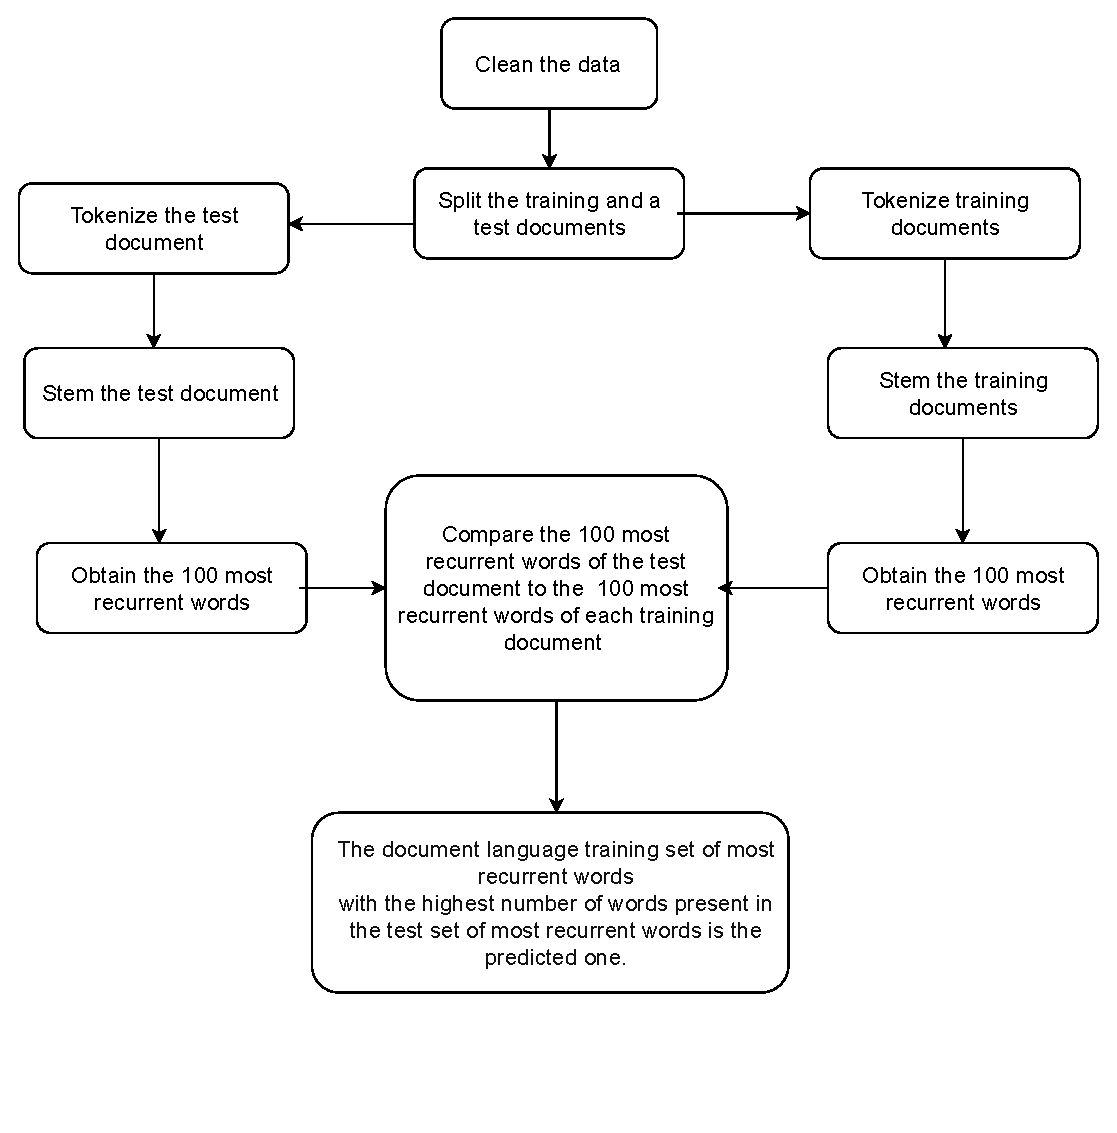
\includegraphics[width=.9\textwidth]{images/native-learn-flowchart.eps}
        \caption{The figure shows how the classification method works.}
        \label{fig:Fig1}
    \end{figure}

    \section{Self Organised Map}\label{sec:som}
    The self-organized maps (SOM) are a type of feed-forward neural network~\cite{58325}. As in human brains, we have several map areas, which react to a specific input data pattern, SOM maps also perform a similar task~\cite{58325}.

    Besides, an ANN is a collection of neurons, where each one holds a set of weights and activation function. It also is part of the SOM which randomly initialize a group of neurons which one with an arrangement of weights~\cite{58325}. It generally has a rectangular or hexagonal format which brings the idea of a map of neurons. The fundamental purpose is that, as long as, the SOM receives an input pattern, a group of specific neurons will react to it. It means that the weights of such neurons suit the input pattern making the neurons activate.

    Even though we already have the main fundamental of the SOM, we can't ignore that neurons in different areas can respond to the same or similar input pattern. Consequently, the neurons compete with each other to decide the one that will represent the input ~\cite{58325}. The comparison between the neuron's output will show the best match.
    Besides, the neurons also have an influence area. We define that area by a specific function ~\cite{58325}. We can, for example, use the Gaussian function to obtain how much influent is each neuron. Therefore, we train the SOM network until obtaining the winners for each data point.

    Finally, after training a SOM we obtain a final map of the distribution of the inputs and its influence area~\cite{58325}.
    Consequently, we used a SOM to show the separability of the languages using as input features the most frequent tokens (stems) of each language (see~\ref{subsec:som-experiment}).

    \section{Experiments}\label{sec:results}

    The experiment consisted of separating the data in training (category profile) and test sets in different folds as it is showed further in this section.
    The evaluation process simply identified whether the classifier predicts correctly or not a given language text document. The table~\ref{tab1}, is the result of the first trial using only one book of the New Testament. We computed separately the stems for each language and then, we saved them in a \textit{.csv} file. After, we used the stems to pre-process the input text and compute the language profile of each language.

    \begin{center}
        \begin{tabular}{ ||c c | c c || }
            \hline
            Language & Match rate & Language & Match rate\\
            \hline
            Apalaí &  0.78 & Kaiwá &  0.83 \\
            Apinayé &  0.9 & Karajá & 0.8 \\
            Apurinã &  0.77 & Kayabí & 0.86 \\
            Bakairi &  0.8 & Kaigáng &  0.82 \\
            Guajajara &  0.82 & Karajá & 0.8 \\
            Guarani Mbyá &  0.82 & Kayabí & 0.86 \\
            Kadiwéu &  0.77 & kayapó &  0.84 \\
            Kagwahiva & 0.83 & Macushi &  0.84 \\
            Kaigáng &  0.82 & Maxakalí & 0.86 \\
            Kayabí & 0.86 & Mundurukú  & 0.79\\
            Nadëb & 0.86 & Nambikuára & 0.92 \\
            Parecis & 0.78 & Paumarí &  0.84\\
            Português & 0.77 & Rikbaktsa &  0.84\\
            Sateré-Mawé & 0.83 & Terena & 0.83\\
            Tukano &  0.85 & Urubu-Kaapor &  0.78\\
            Xavánte & 0.92\\
            \hline
        \end{tabular}
    \end{center}

    Our method could identify correctly all the language, but with different similarities between the training and test set.

    \begin{figure}[ht!]
        \centering
        \includegraphics[width=.9\textwidth]{images/mean.pdf}
        \caption{The figure shows how the behaviour of the match rate through the tests.}
        \label{fig:Fig2}
    \end{figure}
    \subsection{Threshold}\label{subsec:threshold}

    Another approach was to verify the behaviour of our method in different train sets. We increased the size of the train set systematically inserting one book of the Gospels of the New Testament each iteration. We started with one book and ending with four, the reaming books were considered as the test set. The result found in figure 2 shows the relation between the mean of the number of words and the performance. The performance is given by the mean of match accuracy between the top-ranked words in the test and training set. Again method predicts correctly all the languages.

    \begin{center}
        \begin{tabular}{ ||c c c c || }
            \hline
            Number of Books &  Match rate & Standard Deviation & Time~(secs)\\ [0.5ex]
            \hline\hline
            1 &  0.82777 & 0.04148 & 217.74571\\
            2 &  0.81555 & 0.04669 & 202.51046\\
            3 &  0.79518 & 0.04557 & 174.92763\\
            4 &  0.79296 &  0.04503 & 161.29179\\
            \hline
        \end{tabular}
    \end{center}
% Falar das especificações do hardware e realizar novos teste.

    \subsection{SOM Network Experiment}\label{subsec:som-experiment}
    \section{Discussion}\label{sec:discussion}

    Throughout this paper, we tried to develop the idea of an ideal language identifier algorithm to classify indigenous Brazilian Languages.
    We consider a significant three main features that the algorithm must hold. The first characteristic was the no a priori knowledge about the language, which is the same concern of the textCat work ~\cite{cavnar1994n}.

    Besides, the second feature considers the small amount of text corpus.
    Further, the third characteristic was the concern about the performance despite the method simplicity. The method makes use of only terms frequency, as features and not other ones like n-grams rate.
    Further, the results outcomes seem to be excellent in this primarily study.
    We obtained comparable results with the state of the art work~\cite{cavnar1994n}, having 100\% hits.

    Besides the good results, we also hold key differences, one of them was the use of an automatic method to extract the n-grams.
    The works in~\ref{sec:background-work}, used a pre-defined extraction method taking only and prefix or only the suffix or any possible n-gram\cite{cavnar1994n},~\cite{gomez2017discriminating}.
    However, we chose to use an algorithm to detect the best stems of each language.
    It allowed us to have a better n-gram profile picture of each language.
    Further, we avoid using linear methods such as SVM and Linear Regression~\cite{gomez2017discriminating}.

    Therefore, we did not have any concern related to limitation due to the data dimension. Moreover, since, we have an efficient method we did not use techniques using ANN, it empowers us to have a simple and faster method~\cite{kp2019deep}.


    \section{Conclusion}\label{sec:conclusion}

    The method opens the exploration of the classification of native languages with a few text corpus and, no apriori knowledge, creating a language profile to identify them. As in the original approach of textCat, we also obtain considerable results.

    Finally, Some of the limitations are still the need for computing the stemming of word, even though this process is language-independent. Further, we can explore the use of the technique to categorize language dialects and more co-related languages.


    \section*{Acknowledgment}

    We thanks everyone involved in the translation of the bible for the 26 Brazilian native languages and their availability at \cite{angelo} which made this work possible.

    \bibliographystyle{splncs04}
    \bibliography{sbc-template}


\end{document}
